\newpage
\subsection{Calcul de la couleur à afficher}
\subsubsection{Calcul de normale}
Pour les calculs de couleurs, on va avoir besoin de la normale $\Vec{N}$ de la surface de l'objet "rencontré" par le rayon.
\begin{align*}
    \Vec{N}=normalize(\Vec{\nabla}SDF\_Scene(P))
\end{align*}
avec $normalize(\cdot )=\frac{\cdot }{\|\cdot \|}$\\
\\
\textbf{Remarque} : on utilise le fait que $SDF\_Scene$ est $\mathcal{C}^1(\mathbb{R}^3,\mathbb{R})$ sauf en certains points particuliers, comme par exemple à l'interieur d'un plan sans volume. Cependant, ces points critiques sont négligeables par rapport au volume total des objets. On évitera d'utiliser certaines figures, au profit d'autres ayant moins de discontinuités. Par exemple, on préférera utiliser un pavé très fin plutôt qu'un plan en deux dimensions.

\subsection{Calcul des ombres}
Pour determiner s'il y a une ombre à un point $P$, il suffit de projeter un rayon d'origine $P$ et de direction $Sun\_Direction$ de la même manière que dans la partie \ref{subsec:projection} \nameref{subsec:projection}. Si le rayon projetté converge, alors il a rencontré un obstacle et il y a une ombre. Sinon, il n'y a pas d'ombre.\\
\\\textbf{Remarque:} Le calcul des ombres est couteux en ressources.

\subsubsection{Calcul de l'éclairage}
On pose $LightPos \in \mathbb{R}^3$ la position d'une source de lumière et $LightColor$ sa couleur.
\\La contribution de cette source de lumière à l'éclairement d'un objet blanc de normale $\Vec{N}$ au point $\mathbf{P}$ est donnée par ce calcul :
$$
    Contribution=\left\{
        \begin{array}{ll}
            0 & \mathbf{si\ P\ est\ dans\ l'ombre} \\
            max(\left\langle \Vec{N},\ normalize(Lightpos-P) \right\rangle,\ 0) \times LightColor & \mathbf{sinon}
        \end{array}
    \right.
$$
\textbf{Remarque} : S'il y a plusieurs sources de lumière, il suffit de sommer la contribution de chacune de ces sources. Il n'est pas necessaire de gerer d'éventuel problème de dépassement de couleur car le shader le fait lui-même.

\newpage
\subsubsection{Calcul de la couleur de l'objet}

La couleur des objets est donnée par une valeur comprise entre 0 et 360 degrés. La valeur correspond à la teinte de l'objet. Comme montré sur le schéma ci-dessous une valeur à 180 degrés (donc au milieu) correspondrait à du cyan.

\begin{figure}[h]
    \centering
    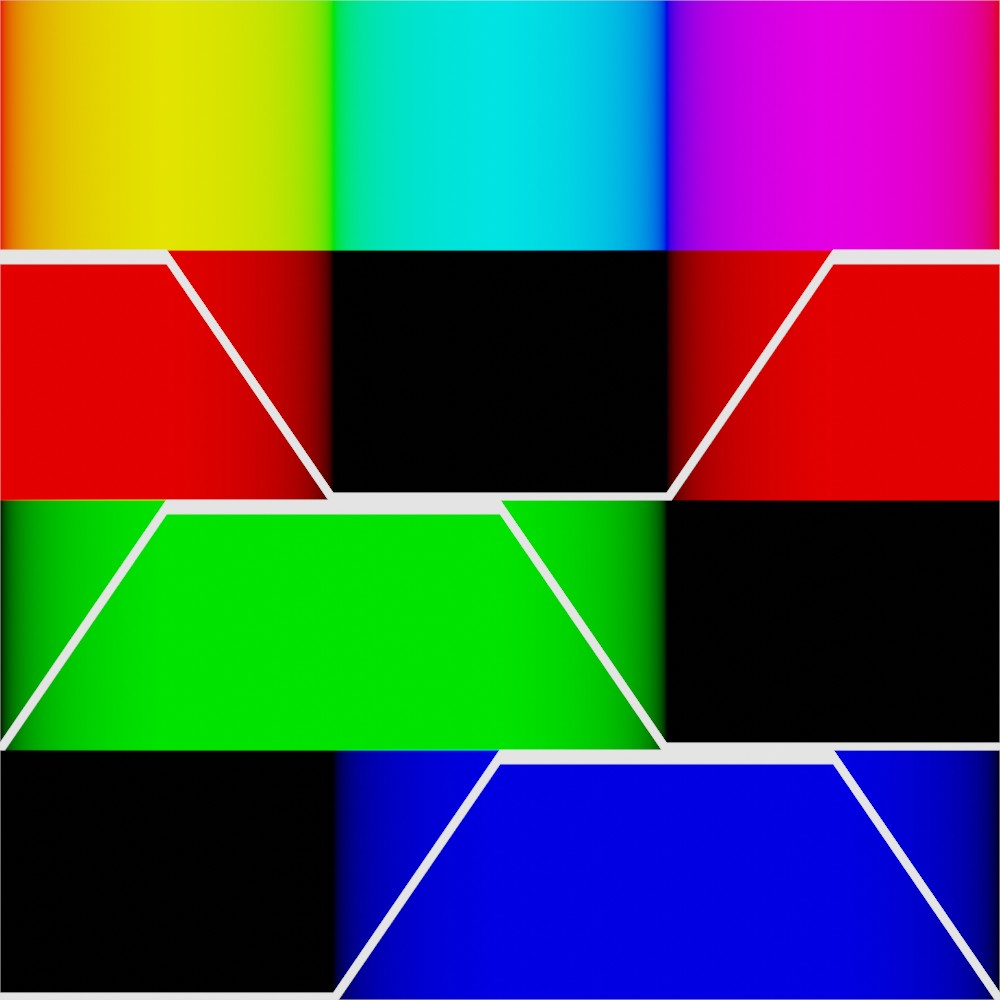
\includegraphics[width=8cm]{images/huetorgb.jpg}
    \caption{Décomposition de la couleur }\label{fig:huetorb}
\end{figure}

On remarque que l'on peut facilement calculer les valeurs de rouge, de vert et de bleu (comprises entre 0 et 1) nécessaires à l'obtention de la coueleur souhaitée.\\
En effet, il suffit de découper la courbe tous les 60 degrés et on obtient des courbes constantes ou linéaires.\\
Pour reprendre l'exemple du cyan, en se plaçant à 180 degrés on remarque que le rouge vaut 0 et que le bleu et le vert valent 1.

% \subsection{Calcul de reflexion}
% Pour rajouter des surfaces reflechissantes au moteur 3D, il faut pouvoir calculer des reflexions. Cela est faisable avec les calculs suivants :
% \begin{align*}
%     \Vec{direction} &= \Vec{D}-2*\left\langle \Vec{D},\Vec{N}\right\langle \time \Vec{N}
%     Couleur
% \end{align*}

\subsection{Calcul final de la couleur d'un pixel}
Il faut finalement combiner tous ces calcul de manière à obtenir la couleur finale à afficher. Voici le calcul de la couleur apparente d'un point $P$ d'un objet de couleur $CouleurObjet$ :
\begin{align*}
    Couleur\_Pixel=min(CouleurObjet,Couleur\_Eclairage)%+reflexion
\end{align*}
avec $min(\Vec{u},\Vec{v})=(min(u_x,v_x),min(u_y,v_y),min(u_z,v_z))$